\documentclass[12pt]{article}
\textwidth=6.35in   
\topmargin=-.05in
\oddsidemargin=0.1in
\textheight=8.45in
\headheight=15pt
\renewcommand{\baselinestretch}{1.4} %line spacing - set to 2 for doublespaced
\usepackage{graphicx} % for easy postscript figure inclusion.
\usepackage[space]{grffile}
\usepackage{url}
\usepackage{fancyhdr}
\usepackage{float}
\usepackage{authblk}
%\usepackage[sort&compress]{natbib}
\usepackage[superscript]{cite}
\usepackage{amsmath, amsthm, amssymb}
\pagestyle{fancy}

\usepackage{xcolor}

\begin{document}
	
	\pagenumbering{arabic}
	
	\url{https://resistorcolorcodecalc.com/}
	
	\section{Introduction}
	
	
	\noindent $\bigcirc$ Objective: 
	
	\noindent $\bigstar$ Bonus: 
	
	\subsection{Program}
	
	Arduino is a small electronics board that is used to obtain measurements from sensors, like a light detector, and send commands to actuators, like motors. They are incredibly capable pieces of equipment. The challenge that we often find when programming is that computers do exactly what we \textbf{\textit{tell}} them to, not what we \textbf{\textit{want}} them to. This can be very frustrating at times. To help avoid confusion, it is beneficial to write down step-by-step what we want the program, or equipment, to do. I'll try to help you by providing this process in the beginning but you will need to do this yourself later. If you run into problems, a great first step for diagnosing issues is to compare what you program/Arduino is actually doing versus what you expected with your written out procedure.
	
	\subsection{Arduino Requirements}
	
	All Arduino programs will have two functions in them.
	
	The first function is called \textbf{setup}. This runs right at the very beginning when the Arduino first starts up and is used for configuration. The online process we will use to make programs will actually take care of most of this for us.
	
	The second function is called \textbf{loop}, it runs after \textbf{setup} and it runs over and over again in a loop. This is where you will put all of your instructions that you want the program/Arduino to do.
	
	\begin{figure}[H]
		\begin{center}
			%\title{}
			
\includegraphics[scale=0.7]{p_minimal_program}
			\caption{Example of the minimal required functions for an Arduino program.}
			\label{prog:minimal_program}
		\end{center}
	\end{figure}
	
	\section{LED Basics}
	
	An LED, light emitting diode, is an electrical component that produces light. We will be using these to gain a better understanding of circuits and programming.
	
	LEDs have two leads, or wires. The longer lead is the anode and gets connected to the positive side of a power source. The shorter lead is the cathode and is connected to the negative side of a power source. LEDs must always be connected this way. If your LED does not light up as you expect, try reversing it.
	
	LEDs cannot control how much current flows through them so we must always have a resistor in series with the LED. If there is no resistor in the circuit with the LED then something will get wrecked, either the LED or the power source, the Arduino in this case.
	
	\subsection{Circuit}
	
	Try connecting an LED up in a circuit as shown in figure \ref{fig:circuit_simple}.
	
	\textcolor{red}{Add some notes to describe the circuit. Consider the diode is polar.}
	
	\begin{figure}[H]
		\begin{center}
			%\title{}
			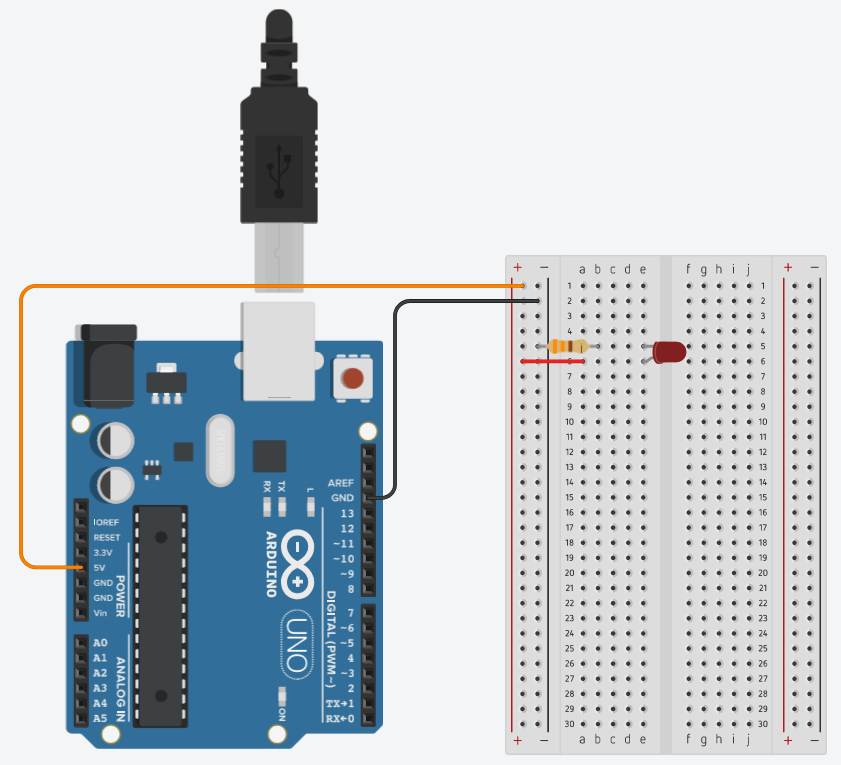
\includegraphics[scale=0.5]{LED_simple}
			\caption{Circuit diagram to directly power the LED.}
			\label{fig:circuit_simple}
		\end{center}
	\end{figure}

	\subsection{Program}
	
	There is no programming required for this circuit. The Arduino has no control over any of the pins we are using and all it does is provide power.
	
	\textcolor{red}{What is the purpose of this section? \\ How many sections do you plan to go through a day?}
	
	\subsection{Objectives}
	
	\noindent $\bigcirc$ Objective: Power an LED.
	
	\noindent $\bigstar$ Bonus: What happens when the LED is plugged in backwards?
	
	\indent $\bigstar$ What happens when the order is reversed and the LED is connected to ground and the resistor is connected to power?
	
	
	
	
	
	\section{Blink}
	
	Now that we have an LED that lights up, lets try to automate it to blink. We will do this with a digital pin which we can turn on and off.
	
	\subsection{Circuit}
	
	Connect the circuit as shown in figure \ref{fig:circuit_blink}. An important thing to notice as this point is that the LED will now be controlled by pin 11 and not the 5V pin.
	
	\textcolor{red}{Comment on the required resistor value}
	
	\begin{figure}[H]
		\begin{center}
			%\title{}
			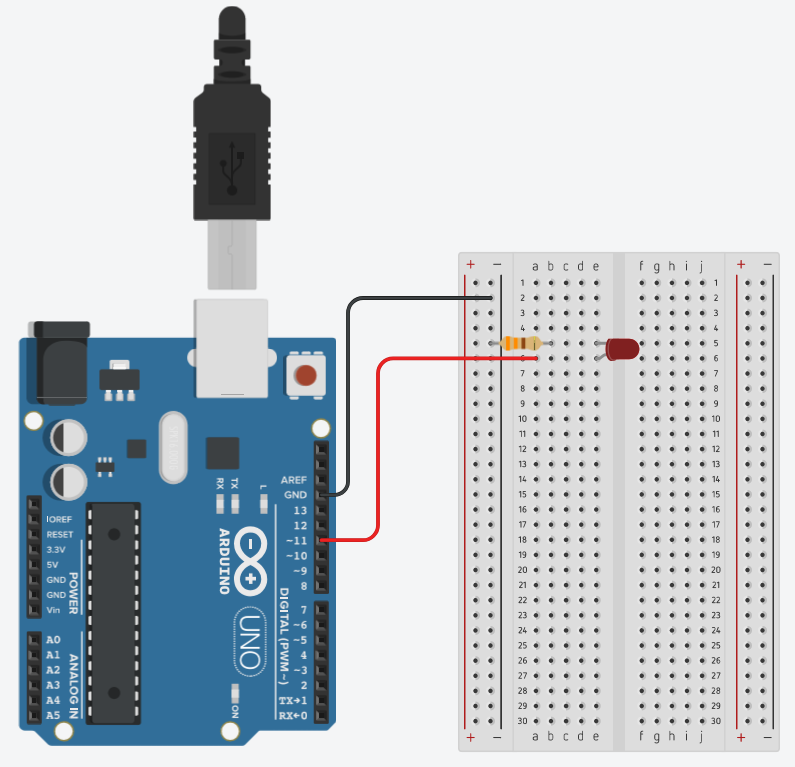
\includegraphics[scale=0.5]{blink_circuit}
			\caption{Circuit diagram for the basic LED blink program.}
			\label{fig:circuit_blink}
		\end{center}
	\end{figure}

	\subsection{Program}
	
	The process to automate the on/off sequence of the light is:
	
	\begin{enumerate}
		\itemsep -1em
		\item Turn the LED on by setting pin 11 to ON
		\item Delay some amount of time that we want the LED to be on
		\item Turn the LED off by setting pin 11 to OFF
		\item Delay for the time we want the LED to be off
	\end{enumerate}

	I will provide you with an example of how to make this process work. Compare the above process with how the code blocks are setup. In this case, the program is set to wait 500 milliseconds, or half of a second, after the LED is switched on or off.
	
	\begin{figure}[H]
		\begin{center}
			%\title{}
			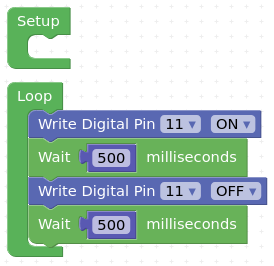
\includegraphics[scale=0.7]{p_blink}
			\caption{Program to automatically blink an LED.}
			\label{prog:blink}
		\end{center}
	\end{figure}
	
		
	\subsection{Functions}
	
	Functions are a simple way to take a specific process, like the previous steps to turn an LED on and off, and make it easy to use. Functions also help make code easier to read, build, maintain and fix.
	
	Look at this example, Figure \ref{prog:blink_function}. It has the exact same process and outcome as our blink program except the steps to blink an LED are in a function and we refer to that function when we want the blink process to run.
	
	\begin{figure}[H]
		\begin{center}
			%\title{}
			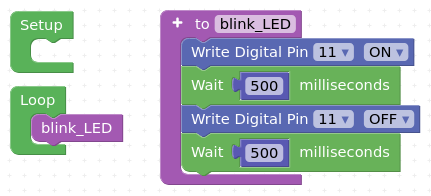
\includegraphics[scale=0.7]{p_blink_function}
			\caption{Example program to blink an LED using a function.}
			\label{prog:blink_function}
		\end{center}
	\end{figure}

	%Do you see how this is easier to read?
	When the Arduino is running it will \textbf{blink the LED}. If we want to see the exact process of how Arduino controls the LED and causes it to blink, we can look at the function \textbf{blink\_LED}.
	
	%Imagine if we had 3, 10, or even a 100 LEDs to control. The \textbf{loop} function would get very confusing very quickly!
	
	It should be noted that you have been using functions already. Both \textbf{Write Digital Pin} and \textbf{Wait} are functions that are built-in to the Ardiuno system. These functions also have required input values. For \textbf{Write Digital Pin} you must provide the pin number that you want to make a change to and the new value that you want it to have. %These functions help to make your life much easier as you do not need to understand what they are doing on a step-by-step level, you only need to know what they accomplish in the end.
	
	
	
	\subsection{Objectives}
	
	\noindent $\bigcirc$ Objective: Program the Arduino to switch the LED on and off.
	
	\noindent $\bigstar$ Bonus: What happens when you vary the amount of time in each of the delay, or \textbf{Wait}, blocks?
	
	\indent $\bigstar$ Reduce the time in each delay block to be less than 15 microseconds each. Can you still see the LED flash?
	
	\textcolor{red}{The objective is awkward and should be restated}
	\indent $\bigstar$ Keep the total sum of time in each delay block to be 15 microseconds while changing the time in each delay block. For example, 3 and 12 microseconds? 5 and 10? 7 and 8? 12 and 3?
	
	
	
	
	
	
	\section{Traffic Lights}
	
	\begin{figure}[H]
		\begin{center}
			%\title{}
			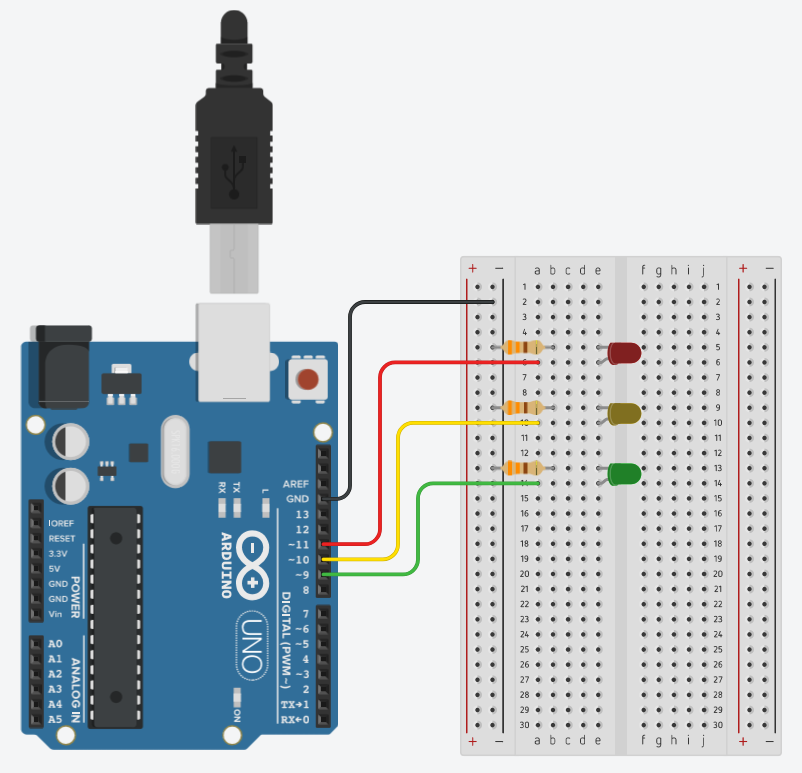
\includegraphics[scale=0.5]{traffic_light}
			\caption{Circuit diagram for the traffic lights program.}
			\label{fig:circuit_traffic_light}
		\end{center}
	\end{figure}
	
	\subsection{Process}
	
	Traffic lights have a very simple process that they run through.
	
	\begin{enumerate}
		\itemsep -1em
		\item Go - red off \& green on
		\item Caution - green off \& yellow on
		\item Stop - yellow off \& red on
	\end{enumerate}
	
	\subsection{Programming}
	
	Using the program you made to blink an LED (use the version which has the \textbf{blink\_LED} function) as an example, try to make a new program for the traffic lights. Make a function for the red LED, another for the green and a third for the yellow LED.
	
	Do you get the result that you are expecting? Remember, real traffic lights never have all 3 lights off at the same time. This would cause confusion and people may not know what they are supposed to be doing if no light is on. Do you always have one LED being lit up?
	
	
	 %\textcolor{red}{Is this a good time to introduce buttons?}
	
	
	\section{Controlling LED Brightness}
	
	Controlling the brightness of an LED can be done in two different ways. The first way is to change the amount of current flowing through it using a resistor. The second method is actually a trick played on your eye, but we'll discuss this in section \ref{ssec:PWM intro}.
	
	\subsection{Resistors: Reducing current flow}
	
	\textcolor{red}{What is current?}
	
	Resistors are an electrical device that reduce the amount of current flowing through a circuit. Since LEDs are unable to control the amount of current that flows through them, a resistor is always using to limit current flow. We can use this to our advantage to change how bright an LED is since the more current that flows through an LED, the brighter it is.
	
	\textcolor{red}{What is a circuit?}
	
	The following circuit uses a potentiometer, or pot, which is simply a resistor that we can change the resistance of the circuit. We will leave the resistor in the circuit that we were using before in place and add the potentiometer.
	
	\begin{figure}[H]
	\begin{center}
		%\title{}
		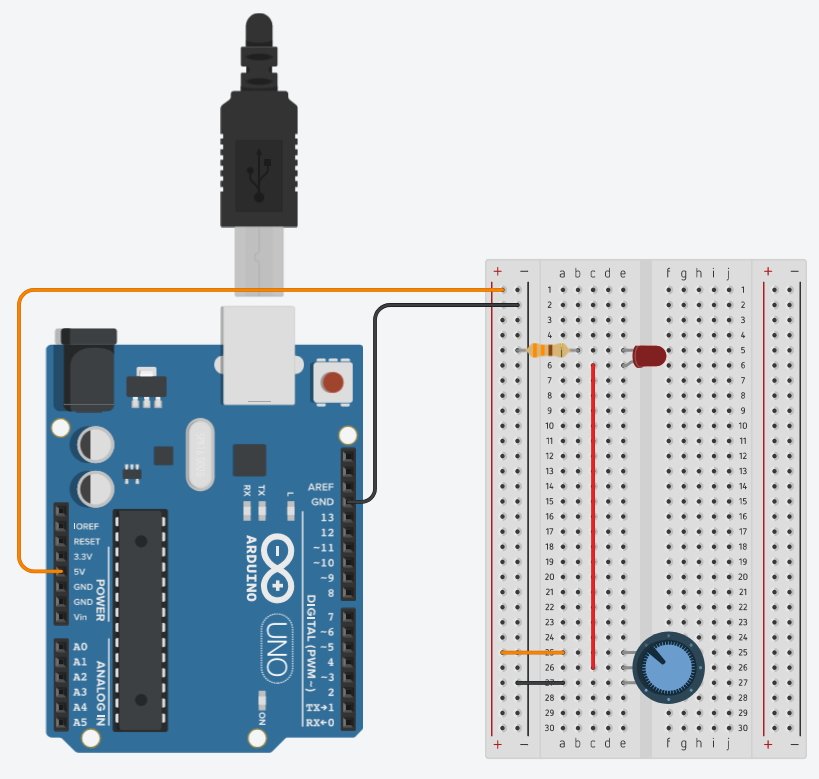
\includegraphics[scale=0.5]{LED_brightness_pot}
		\caption{Circuit diagram for the traffic lights program.}
		\label{fig:circuit_pot_brightness_ctrl}
	\end{center}
	\end{figure}

	The circuit uses the Arduino to power the LED only and no programming is required.
	
	When you turn the dial on the potentiometer, the LED will get brighter as the resistance of the potentiometer decreases and more current flows. If you turn the dial the other way, the resistance of the potentiometer will increase, reducing current flow and the LED will get dimmer.
	
	
	\textcolor{red}{Is this a good time to do the Analog read process to show how LEDs turn on at specific voltages? Serial communication introduction?}
	
	
	
	\subsection{PWM: On/Off really fast!}
	\label{ssec:PWM intro}
	
	The previous method used hardware and actually caused the LED to get brighter and dimmer. This second method will use software to achieve the same goal but this time it will only make the LED appear brighter or dimmer using an optical trick.
	
	\subsubsection{Circuit}
	
	First lets set up the circuit. You'll notice that we are still using the potentiometer. However, rather than using the potentiometer to directly control the LED, we will use the Arduino to make a measurement of the potentiometer's value.
	
	\begin{figure}[H]
		\begin{center}
			%\title{}
			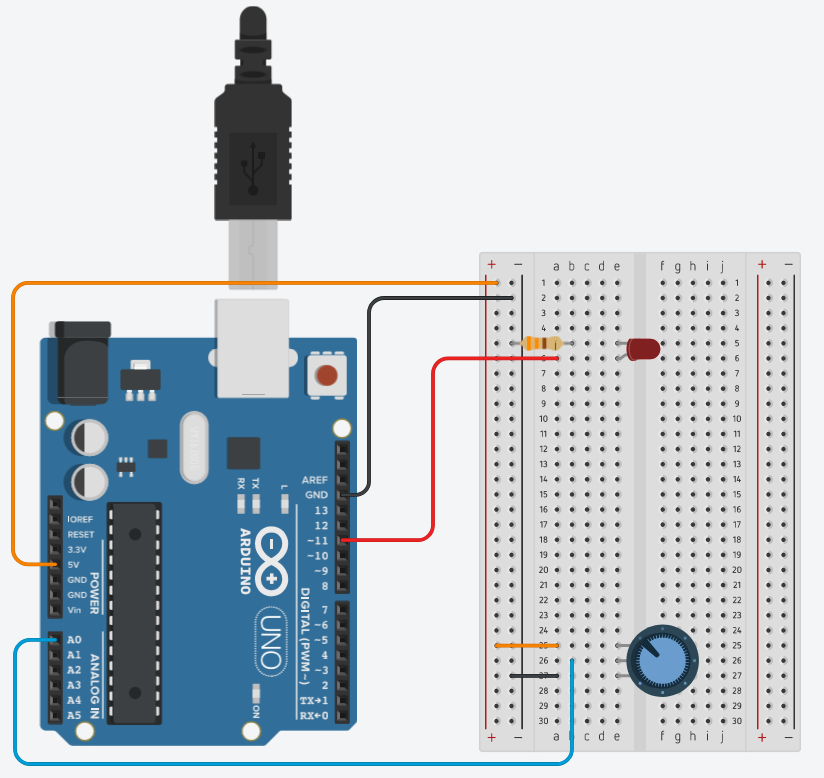
\includegraphics[scale=0.5]{LED_brightness_pwm}
			\caption{Circuit diagram for the traffic lights program.}
			\label{fig:circuit_pwm_brightness_ctrl}
		\end{center}
	\end{figure}

	\subsubsection{PWM Signals}
	
	On the Arduino board you will see a little $\sim$ mark next to some of the pin numbers. \textcolor{red}{(There should be a diagram/image to show this. Reference a nearby figure as the arduino is there?)} This $\sim$ indicates that the pin can be used to output a Pulse Width Modulated signal, or PWM signal.
	
	Remember at the beginning we made a program to blink the LED on and off repeatedly? That basically all a PWM signal is, turning a signal on and off. The difference is that we are now going to turn the light on and off really, really fast. Like, 480 times every second fast. The only control that we have over the PWM signal is the percent of time that the signal is on vs off.
	
	\subsubsection{Program}
	
	The process that we need for this program is:
	
	\begin{enumerate}
		\itemsep -1em
		\item Read the value of the potentiometer using \textbf{Read Analog Pin}
		\item Optional: Send the potentiometer value back to the computer using serial so we can see what the Arduino knows
		\item Use the \textbf{Map} function to get an acceptable PWM value
		\item Update the PWM signal that is output using \textbf{Write Analog (PWM)}
	\end{enumerate}

	
	\begin{figure}[H]
		\begin{center}
			%\title{}
			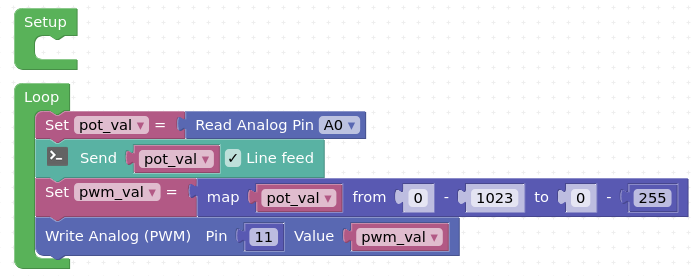
\includegraphics[scale=0.7]{p_pwm_led_ctrl}
			\caption{PWM LED brightness control program.}
			\label{prog:pwm_led_ctrl}
		\end{center}
	\end{figure}


	\subsubsection{Map - Built in Function}
	
	Note: How the \textbf{Map} function works in not important at this time. You are free to skip this section and simply use the values that are provided in the program we make for this section.
	
	\textbf{Map} is a built in function that Arduino has by default and it requires some input values and it returns a result. We don't need to know how it works specifically, we just to know what it does over all. The inputs of \textbf{Map}, in order, are:
	
	
	
	\begin{itemize}
		\itemsep -1em
		\item value - A number that we to convert from one range A to range B
		\item fromLow - The lower end of range A
		\item fromHigh - The upper end of range A
		\item toLow - The lower end of range B
		\item toHigh - The upper end of range B
	\end{itemize}

	\begin{figure}[H]
	\begin{center}
		%\title{}
		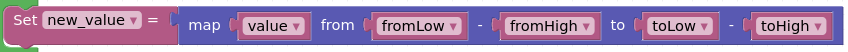
\includegraphics[scale=0.5]{MAP_parameters}
		\caption{\textbf{map} function form.}
		\label{fn:MAP_parameters}
	\end{center}
	\end{figure}

	\textbf{Map} is a function that returns a value. In the example above, we are going to store the result of \textbf{map} in a variable called \textbf{new\_value}.
	
	For example, lets say you take a test and get a score, value, of 10. The minimumm score, fromLow, that you can get is 0 and the maximum score, from High, is 20. We can \textbf{Map} your score to a percent with a minimum percent, toLow, of 0\% and a maximum percent, toHigh, of 100\%. \textbf{Map} will return a value of 50.
	
	
	
	\section{Serial Communication}
	
	A helpful diagnostic method.
	
	
	
	
	
	%\newpage
	%\begin{thebibliography}{1}
	%\end{thebibliography}
	
\end{document}


%4.1
%4.2
%5.1 - diagram
%5.2.3
%5.2.4



















%Outline for function calls

%\begin{figure}[H]
%\begin{center}
%\title{}
%\includegraphics[scale=0.7]{HallEffect}
%\caption{Diagram showing current flow and build up of charge due to electric and magnetic %fields.\cite{Fitzpatrick}}
%\label{fig:pic}
%\end{center}
%\end{figure}

%\begin{equation} \label{eq:Lorentz}
%\vec{F}=q(\vec{E}+\vec{v} \times \vec{B})
%\end{equation}

%\cite{memoir}
%\ref{eq:Lorentz}

%\bibitem{memoir} Bridgman, P. W. "Biographical Memoir of Edwin Herbert Hall." BIOGRAPHICAL MEMOIRS (n.d.): 79-82.  \url{http://www.nasonline.org/publications/biographical-memoirs/memoir-pdfs/hall-edwin.pdf}. Web. 11 Apr. 2015.
